% TikZ schematics for len52.tex.  Each macro draws one figure body.
\tikzset{
  knot/.style={line width=1.5pt, line cap=round, line join=round},
  edge/.style={line width=1.5pt, line cap=round, color=black!85},
  new/.style={line width=1.5pt, line cap=round, color=red!70!black},
  ghost/.style={line width=0.6pt, dashed, color=black!45},
  vtx/.style={circle, fill=black, inner sep=1.4pt},
  free/.style={circle, draw=black, fill=white, inner sep=1.4pt, line width=0.6pt},
  site/.style={circle, draw=red!70!black, fill=white, inner sep=1.6pt, line width=0.9pt},
  lbl/.style={font=\footnotesize},
  tri/.style={fill=blue!12},
  tri2/.style={fill=orange!18},
  mv/.style={-{Stealth[length=2.2mm]}, line width=0.7pt, color=red!70!black},
  stp/.style={-{Stealth[length=2.6mm]}, line width=0.7pt},
}
\tikzset{iso/.style={x={(1cm,0cm)},y={(0.42cm,0.30cm)},z={(0cm,1cm)}}}

% ---------------------------------------------------------------- Delta-move
\newcommand{\FigDelta}{%
\begin{tikzpicture}[scale=1.0]
\begin{scope}
  \fill[tri] (0,0) -- (2,0) -- (1.1,1.25) -- cycle;
  \draw[knot] (-0.9,-0.7) .. controls (-0.5,-0.2) .. (0,0) -- (2,0) .. controls (2.5,0.2) .. (2.9,0.8);
  \draw[knot] (-0.6,1.9) .. controls (0.6,2.3) and (1.8,1.7) .. (2.8,2.1);
  \node[vtx] at (0,0) {}; \node[vtx] at (2,0) {};
  \node[lbl,below] at (0,-0.05) {$a$}; \node[lbl,below] at (2,-0.05) {$b$};
  \node[free] at (1.1,1.25) {}; \node[lbl,above left] at (1.1,1.25) {$c$};
  \node[lbl] at (1,-0.75) {(a) before};
\end{scope}
\draw[stp] (3.15,0.5) -- (3.85,0.5);
\begin{scope}[xshift=4.9cm]
  \fill[tri] (0,0) -- (2,0) -- (1.1,1.25) -- cycle;
  \draw[ghost] (0,0) -- (2,0);
  \draw[knot] (-0.9,-0.7) .. controls (-0.5,-0.2) .. (0,0) -- (1.1,1.25) -- (2,0) .. controls (2.5,0.2) .. (2.9,0.8);
  \draw[knot] (-0.6,1.9) .. controls (0.6,2.3) and (1.8,1.7) .. (2.8,2.1);
  \node[vtx] at (0,0) {}; \node[vtx] at (2,0) {}; \node[vtx] at (1.1,1.25) {};
  \node[lbl,below] at (0,-0.05) {$a$}; \node[lbl,below] at (2,-0.05) {$b$};
  \node[lbl,above left] at (1.1,1.25) {$c$};
  \node[lbl] at (1,-0.75) {(b) after};
\end{scope}
\begin{scope}[xshift=10.0cm]
  \fill[tri] (0,0) -- (2,0) -- (1.1,1.25) -- cycle;
  \draw[knot] (-0.9,-0.7) .. controls (-0.5,-0.2) .. (0,0) -- (2,0) .. controls (2.5,0.2) .. (2.9,0.8);
  \draw[knot] (0.70,-0.9) -- (0.76,0.40);
  \draw[knot,densely dotted] (0.76,0.40) -- (0.80,1.0);
  \draw[knot] (0.80,1.0) -- (0.86,2.2);
  \node[circle,fill=red!70!black,inner sep=1.3pt] at (0.765,0.5) {};
  \node[vtx] at (0,0) {}; \node[vtx] at (2,0) {};
  \node[lbl,below] at (-0.05,-0.05) {$a$}; \node[lbl,below] at (2,-0.05) {$b$};
  \node[lbl,right] at (1.35,1.25) {$c$}; \node[free] at (1.1,1.25) {};
  \node[lbl,align=center] at (1,-1.15) {(c) not allowed: another\\ part of $K$ pierces $abc$};
\end{scope}
\end{tikzpicture}}

% ---------------------------------------------------------------- segment and square
\newcommand{\FigSegSquare}{%
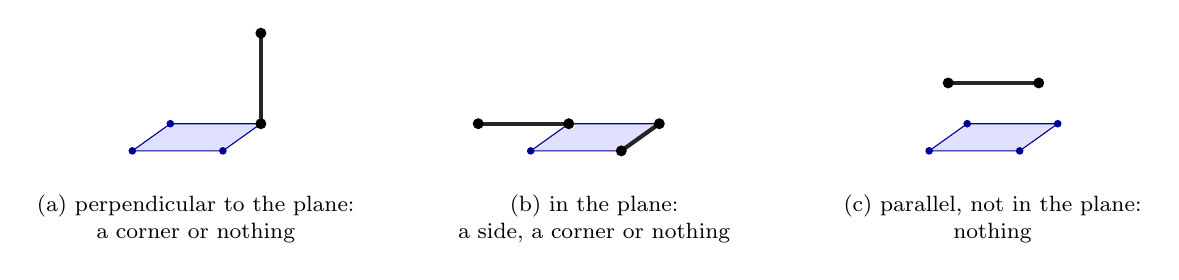
\begin{tikzpicture}[iso, scale=1.15]
\foreach \dx/\cap in {0/{(a) perpendicular to the plane:\\ a corner or nothing}, 4.4/{(b) in the plane:\\ a side, a corner or nothing}, 8.8/{(c) parallel, not in the plane:\\ nothing}} {
\begin{scope}[xshift=\dx cm]
  \fill[blue!12] (0,0,0) -- (1,0,0) -- (1,1,0) -- (0,1,0) -- cycle;
  \draw[thin,blue!60!black] (0,0,0) -- (1,0,0) -- (1,1,0) -- (0,1,0) -- cycle;
  \foreach \p in {(0,0,0),(1,0,0),(1,1,0),(0,1,0)} \fill[blue!60!black] \p circle (1.2pt);
  \node[lbl,align=center] at (0.7,0,-0.75) {\cap};
\end{scope}}
\draw[edge] (1,1,0) -- (1,1,1);
\node[vtx] at (1,1,0) {}; \node[vtx] at (1,1,1) {};
\begin{scope}[xshift=4.4cm]
  \draw[edge] (1,0,0) -- (1,1,0); \node[vtx] at (1,0,0) {}; \node[vtx] at (1,1,0) {};
  \draw[edge] (0,1,0) -- (-1,1,0); \node[vtx] at (-1,1,0) {}; \node[vtx] at (0,1,0) {};
\end{scope}
\begin{scope}[xshift=8.8cm]
  \draw[edge] (0,0.5,0.6) -- (1,0.5,0.6) ; \node[vtx] at (0,0.5,0.6) {}; \node[vtx] at (1,0.5,0.6) {};
\end{scope}
\end{tikzpicture}}

% ---------------------------------------------------------------- corner flip and U-turn removal as two Delta-moves
\newcommand{\FigFlipDelta}{%
\begin{tikzpicture}[scale=1.15]
% row 1: corner flip
\foreach \k in {0,1,2} {
\begin{scope}[xshift=\k*3.6cm]
  \draw[edge] (0,-0.75) -- (0,0); \draw[edge] (1,1) -- (1.75,1);
  \ifnum\k=0 \draw[edge] (0,0) -- (0,1) -- (1,1); \draw[ghost] (0,0) -- (1,0) -- (1,1); \fi
  \ifnum\k=1 \fill[tri] (0,0) -- (0,1) -- (1,1) -- cycle; \draw[ghost] (0,0) -- (0,1) -- (1,1); \draw[edge] (0,0) -- (1,1); \fi
  \ifnum\k=2 \fill[tri2] (0,0) -- (1,0) -- (1,1) -- cycle; \draw[ghost] (0,0) -- (1,1); \draw[edge] (0,0) -- (1,0) -- (1,1); \fi
  \node[vtx] at (0,0) {}; \node[vtx] at (1,1) {};
  \ifnum\k=0 \node[vtx] at (0,1) {}; \node[free] at (1,0) {}; \fi
  \ifnum\k=1 \node[free] at (0,1) {}; \node[free] at (1,0) {}; \fi
  \ifnum\k=2 \node[free] at (0,1) {}; \node[vtx] at (1,0) {}; \fi
  \node[lbl,left] at (-0.05,0) {$v_{i-1}$}; \node[lbl,above left] at (0,1) {$v_i$};
  \node[lbl,above] at (1,1.05) {$v_{i+1}$}; \node[lbl,below right] at (1,0) {$v'$};
\end{scope}}
\node[lbl] at (0.5,-1.15) {(a) $|w|$};
\node[lbl,align=center] at (4.1,-1.2) {(b) first $\Delta$-move:\\ triangle $v_{i-1}v_iv_{i+1}$};
\node[lbl,align=center] at (7.7,-1.2) {(c) second $\Delta$-move:\\ triangle $v_{i-1}v'v_{i+1}$};
\draw[stp] (2.05,0.5) -- (2.75,0.5); \draw[stp] (5.65,0.5) -- (6.35,0.5);
% row 2: U-turn removal
\begin{scope}[yshift=-3.3cm]
\foreach \k in {0,1,2} {
\begin{scope}[xshift=\k*3.6cm]
  \draw[edge] (0,-0.75) -- (0,0); \draw[edge] (1,0) -- (1,-0.75);
  \ifnum\k=0 \draw[edge] (0,0) -- (0,1) -- (1,1) -- (1,0); \draw[ghost] (0,0) -- (1,0); \fi
  \ifnum\k=1 \fill[tri] (0,0) -- (0,1) -- (1,1) -- cycle; \draw[ghost] (0,0) -- (0,1) -- (1,1); \draw[edge] (0,0) -- (1,1) -- (1,0); \fi
  \ifnum\k=2 \fill[tri2] (0,0) -- (1,1) -- (1,0) -- cycle; \draw[ghost] (0,0) -- (1,1) -- (1,0); \draw[edge] (0,0) -- (1,0); \fi
  \node[vtx] at (0,0) {}; \node[vtx] at (1,0) {};
  \ifnum\k<1 \node[vtx] at (0,1) {}; \node[vtx] at (1,1) {}; \fi
  \ifnum\k=1 \node[vtx] at (1,1) {}; \node[free] at (0,1) {}; \fi
  \ifnum\k=2 \node[free] at (0,1) {}; \node[free] at (1,1) {}; \fi
  \node[lbl,left] at (-0.05,0) {$v_{i}$}; \node[lbl,above left] at (0,1) {$v_{i+1}$};
  \node[lbl,above right] at (1,1) {$v_{i+2}$}; \node[lbl,right] at (1.05,0) {$v_{i+3}$};
\end{scope}}
\node[lbl] at (0.5,-1.15) {(d) $|w|$};
\node[lbl,align=center] at (4.1,-1.2) {(e) first $\Delta$-move:\\ triangle $v_iv_{i+1}v_{i+2}$};
\node[lbl,align=center] at (7.7,-1.2) {(f) second $\Delta$-move:\\ triangle $v_iv_{i+2}v_{i+3}$};
\draw[stp] (2.05,0.5) -- (2.75,0.5); \draw[stp] (5.65,0.5) -- (6.35,0.5);
\end{scope}
\end{tikzpicture}}

% ---------------------------------------------------------------- potential example
\newcommand{\PsiPoly}[2]{% #1 = list of vertices (x,z), #2 = heights shown
}
\newcommand{\FigPsi}{%
\begin{tikzpicture}[scale=0.82]
\begin{scope}
  \draw[help lines, black!12] (-0.5,-0.5) grid (3.5,2.5);
  \fill[blue!12] (1,1) rectangle (2,2);
  \draw[edge] (0,0) -- (3,0) -- (3,1) -- (2,1) -- (2,2) -- (0,2) -- (0,0);
  \foreach \p/\h in {(0,0)/0,(1,0)/0,(2,0)/0,(3,0)/0,(3,1)/1,(2,1)/1,(2,2)/2,(1,2)/2,(0,2)/2,(0,1)/1}
     { \node[vtx] at \p {}; }
  \node[free] at (1,1) {};
  \node[lbl,above] at (2,2.05) {$v_6$}; \node[lbl,right] at (3,1) {$v_4$}; \node[lbl,below right] at (2,1) {$v_5$};
  \node[lbl,below] at (0,-0.1) {$v_0$}; \node[lbl,left] at (1,1) {$v'$};
  \draw[mv] (1.92,1.92) -- (1.12,1.12);
  \node[lbl,align=left,anchor=north west] at (-0.55,-0.75) {heights $z(v_0),\dots,z(v_9)$:\\ $0,0,0,0,1,1,\mathbf 2,2,2,1$\\ $\psi_Z=9$};
  \node[lbl] at (1.5,3.0) {(a) before the flip at $v_6$};
\end{scope}
\begin{scope}[xshift=6.2cm]
  \draw[help lines, black!12] (-0.5,-0.5) grid (3.5,2.5);
  \draw[ghost] (2,1) -- (2,2) -- (1,2);
  \draw[edge] (0,0) -- (3,0) -- (3,1) -- (2,1) -- (1,1) -- (1,2) -- (0,2) -- (0,0);
  \foreach \p in {(0,0),(1,0),(2,0),(3,0),(3,1),(2,1),(1,1),(1,2),(0,2),(0,1)} { \node[vtx] at \p {}; }
  \node[lbl,left] at (1,1.05) {$v_6'$};
  \node[lbl,align=left,anchor=north west] at (-0.55,-0.75) {heights:\\ $0,0,0,0,1,1,\mathbf 1,2,2,1$\\ $\psi_Z=8$};
  \node[lbl] at (1.5,3.0) {(b) after: $v_6$ replaced by $v'$};
\end{scope}
\draw[->] (10.4,0) -- (10.4,0.65) node[above,lbl] {$z$};
\draw[->] (10.4,0) -- (11.05,0) node[right,lbl] {$x$};
\end{tikzpicture}}

% ---------------------------------------------------------------- the four corner patterns
\newcommand{\Corner}[8]{% #1 prev vertex, #2 v_i, #3 next, #4 v', #5 caption, #6 axis1 label, #7 axis2 label, #8 effect
\begin{tikzpicture}[scale=1.05]
  \fill[blue!12] #1 -- #2 -- #3 -- #4 -- cycle;
  \draw[edge] ($#1!-0.55!#2$) -- #1 -- #2 -- #3 -- ($#3!-0.55!#2$);
  \draw[ghost] #1 -- #4 -- #3;
  \node[vtx] at #1 {}; \node[vtx] at #2 {}; \node[vtx] at #3 {}; \node[free] at #4 {};
  \draw[mv] ($#2!0.14!#4$) -- ($#2!0.82!#4$);
  \node[lbl] at ($#2!-0.28!#4$) {$v_i$}; \node[lbl] at ($#4!-0.3!#2$) {$v'$};
  \node[lbl] at ($#1!-0.42!#3$) {$v_{i-1}$}; \node[lbl] at ($#3!-0.42!#1$) {$v_{i+1}$};
  \draw[->,thin] (2.3,-0.25) -- (2.3,0.3) node[above,lbl] {#6};
  \draw[->,thin] (2.3,-0.25) -- (2.85,-0.25) node[right,lbl] {#7};
  \node[lbl,align=center,text width=5.2cm] at (0.9,-1.45) {#5\\ #8};
\end{tikzpicture}}
\newcommand{\FigCorners}{%
\begin{tabular}{c@{\hspace{1.2cm}}c}
\Corner{(0,0)}{(0,1)}{(1,1)}{(1,0)}{(1) up, then horizontal}{$z$}{$h$}{$v'$ is one unit lower: $\psi_Z$ drops by 1} &
\Corner{(0,1)}{(1,1)}{(1,0)}{(0,0)}{(2) horizontal, then down}{$z$}{$h$}{$v'$ is one unit lower: $\psi_Z$ drops by 1} \\[4mm]
\Corner{(0,0)}{(0,1)}{(1,1)}{(1,0)}{(3) north, then east or west}{$y$}{$x$}{same height; $v'$ is one unit south: $\psi_Y$ drops by 1} &
\Corner{(0,1)}{(1,1)}{(1,0)}{(0,0)}{(4) east or west, then south}{$y$}{$x$}{same height; $v'$ is one unit south: $\psi_Y$ drops by 1}
\end{tabular}}

% ---------------------------------------------------------------- curtain: k-1 flips then a U-turn removal
\newcommand{\CurtainPanel}[3]{% #1 path, #2 hollow points, #3 caption
\begin{tikzpicture}[scale=0.72]
  \draw[help lines, black!10] (-0.6,-0.4) grid (3.6,1.4);
  \draw[ghost] (-0.9,-0.3) -- (0,0); \draw[ghost] (3,0) -- (3.9,-0.3);
  \draw[edge] #1;
  \foreach \p in #2 { \node[free] at \p {}; }
  \node[lbl,align=center] at (1.5,-1.15) {#3};
\end{tikzpicture}}
\newcommand{\FigCurtain}{%
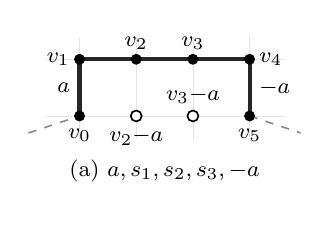
\begin{tikzpicture}[scale=0.72]
  \draw[help lines, black!10] (-0.6,-0.4) grid (3.6,1.4);
  \draw[ghost] (-0.9,-0.3) -- (0,0); \draw[ghost] (3,0) -- (3.9,-0.3);
  \draw[edge] (0,0) -- (0,1) -- (3,1) -- (3,0);
  \foreach \p in {(0,0),(0,1),(1,1),(2,1),(3,1),(3,0)} \node[vtx] at \p {};
  \node[free] at (1,0) {}; \node[free] at (2,0) {};
  \node[lbl,below] at (0,-0.05) {$v_0$}; \node[lbl,left] at (0,1) {$v_1$}; \node[lbl,above] at (1,1) {$v_2$};
  \node[lbl,above] at (2,1) {$v_3$}; \node[lbl,right] at (3,1) {$v_4$}; \node[lbl,below] at (3,-0.05) {$v_5$};
  \node[lbl,below] at (1,-0.05) {$v_2{-}a$}; \node[lbl,above] at (2,0.05) {$v_3{-}a$};
  \node[lbl,left] at (0,0.5) {$a$}; \node[lbl,right] at (3,0.5) {$-a$};
  \node[lbl,align=center] at (1.5,-1.15) {(a) $a,s_1,s_2,s_3,-a$\\ \phantom{x}};
\end{tikzpicture}\hfill
\CurtainPanel{(0,0) -- (1,0) -- (1,1) -- (3,1) -- (3,0)}{{(2,0)}}{(b) flip at $v_1$:\\ $s_1,a,s_2,s_3,-a$}%
\hfill\CurtainPanel{(0,0) -- (2,0) -- (2,1) -- (3,1) -- (3,0)}{{}}{(c) flip at $v_2$:\\ $s_1,s_2,a,s_3,-a$}%
\hfill\CurtainPanel{(0,0) -- (3,0)}{{}}{(d) U-turn removed:\\ $s_1,s_2,s_3$}}

% ---------------------------------------------------------------- DMON3 and DMON4 at the origin
\newcommand{\FigOrigin}{%
\begin{tikzpicture}[iso, scale=1.25]
\begin{scope}
  \draw[edge] (0,0,0) -- (1,0,0); \draw[edge] (0,0,0) -- (0,0,1);
  \draw[edge, densely dashed] (1,0,0) .. controls (2.2,0.2,0.3) and (1.8,0.6,1.9) .. (0,0,1);
  \node[vtx] at (0,0,0) {}; \node[vtx] at (1,0,0) {}; \node[vtx] at (0,0,1) {};
  \node[lbl,below left] at (0,0,0) {$v_0=0$};
  \draw[stp,red!70!black] (0.25,0,-0.12) -- (0.75,0,-0.12); \node[lbl,below,red!70!black] at (0.6,0,-0.12) {$w_0=\mathtt e$};
  \draw[stp,red!70!black] (-0.12,0,0.75) -- (-0.12,0,0.25); \node[lbl,left,red!70!black] at (-0.12,0,0.5) {$w_{n-1}=\mathtt d$};
  \node[lbl,align=center] at (0.9,0,-0.95) {(a) start along $\mathtt e$: $w_0=\mathtt e<\mathtt u=-w_{n-1}$\\ satisfies \dmon4};
\end{scope}
\begin{scope}[xshift=5.0cm]
  \draw[edge] (0,0,0) -- (1,0,0); \draw[edge] (0,0,0) -- (0,0,1);
  \draw[edge, densely dashed] (1,0,0) .. controls (2.2,0.2,0.3) and (1.8,0.6,1.9) .. (0,0,1);
  \node[vtx] at (0,0,0) {}; \node[vtx] at (1,0,0) {}; \node[vtx] at (0,0,1) {};
  \node[lbl,below left] at (0,0,0) {$v_0=0$};
  \draw[stp,red!70!black] (-0.12,0,0.25) -- (-0.12,0,0.75); \node[lbl,left,red!70!black] at (-0.12,0,0.5) {$w_0=\mathtt u$};
  \draw[stp,red!70!black] (0.75,0,-0.12) -- (0.25,0,-0.12); \node[lbl,below,red!70!black] at (0.6,0,-0.12) {$w_{n-1}=\mathtt w$};
  \node[lbl,align=center] at (0.9,0,-0.95) {(b) the same polygon read backwards:\\ $w_0=\mathtt u>\mathtt e=-w_{n-1}$, fails \dmon4};
\end{scope}
\end{tikzpicture}}

% ---------------------------------------------------------------- obligations
\newcommand{\FigObligation}{%
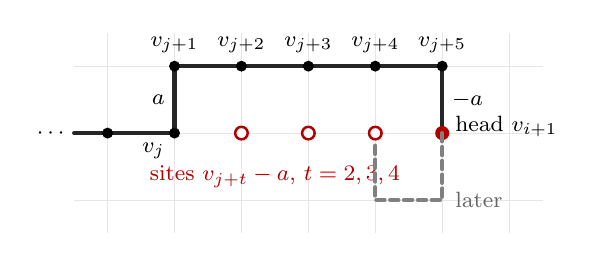
\begin{tikzpicture}[scale=0.85]
  \draw[help lines, black!10] (-1.5,-0.5) grid (5.5,2.5);
  \draw[edge] (-1.5,1) -- (0,1) -- (0,2) -- (4,2) -- (4,1);
  \foreach \p in {(-1,1),(0,1),(0,2),(1,2),(2,2),(3,2),(4,2)} \node[vtx] at \p {};
  \node[circle,fill=red!70!black,inner sep=1.8pt] at (4,1) {};
  \node[lbl,right] at (4.05,1.1) {head $v_{i+1}$};
  \node[lbl,above] at (0,2.05) {$v_{j+1}$}; \node[lbl,below left] at (0,1) {$v_j$};
  \node[lbl,above] at (1,2.05) {$v_{j+2}$}; \node[lbl,above] at (2,2.05) {$v_{j+3}$}; \node[lbl,above] at (3,2.05) {$v_{j+4}$};
  \node[lbl,above] at (4,2.05) {$v_{j+5}$};
  \foreach \p in {(1,1),(2,1),(3,1)} \node[site] at \p {};
  \node[lbl,red!70!black,align=center] at (1.5,0.35) {sites $v_{j+t}-a$, $t=2,3,4$};
  \draw[edge, densely dashed, black!50] (4,1) -- (4,0) -- (3,0) -- (3,0.88);
  \node[lbl,black!60,right] at (4.05,0) {later};
  \node[lbl,left] at (-1.5,1) {$\cdots$};
  \node[lbl,left] at (0,1.5) {$a$}; \node[lbl,right] at (4,1.5) {$-a$};
\end{tikzpicture}}

% ---------------------------------------------------------------- reach test
\newcommand{\FigReach}{%
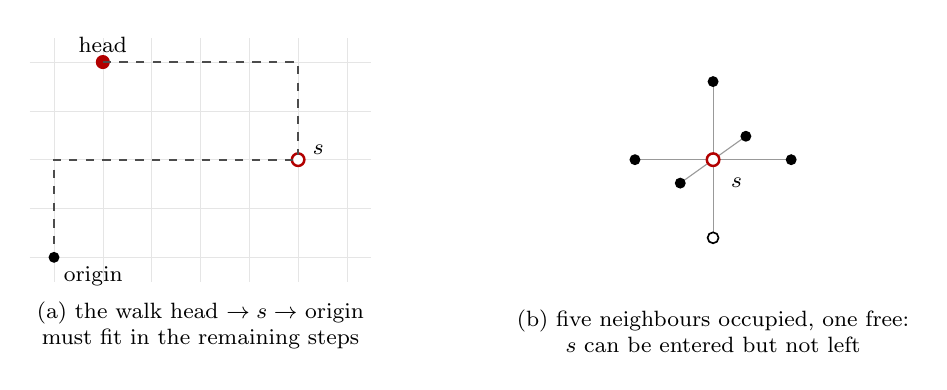
\begin{tikzpicture}[scale=0.62]
\begin{scope}
  \draw[help lines, black!10] (-0.5,-0.5) grid (6.5,4.5);
  \node[vtx] at (0,0) {}; \node[lbl,below right] at (0,0) {origin};
  \node[circle,fill=red!70!black,inner sep=1.8pt] at (1,4) {}; \node[lbl,above] at (1,4) {head};
  \node[site] at (5,2) {}; \node[lbl,right] at (5.1,2.2) {$s$};
  \draw[ghost,black!70] (1,4) -- (5,4) -- (5,2.1);
  \draw[ghost,black!70] (4.9,2) -- (0,2) -- (0,0.1);
  \node[lbl,align=center] at (3,-1.4) {(a) the walk head $\to s\to$ origin\\ must fit in the remaining steps};
\end{scope}
\begin{scope}[xshift=13.5cm,yshift=2cm,iso,scale=1.6]
  \foreach \d in {(1,0,0),(-1,0,0),(0,1,0),(0,-1,0),(0,0,1)} { \draw[thin,black!40] (0,0,0) -- \d; \node[vtx] at \d {}; }
  \draw[thin,black!40] (0,0,0) -- (0,0,-1); \node[free] at (0,0,-1) {};
  \node[site] at (0,0,0) {}; \node[lbl] at (0.3,0,-0.3) {$s$};
  \node[lbl,align=center] at (0,0,-2.2) {(b) five neighbours occupied, one free:\\ $s$ can be entered but not left};
\end{scope}
\end{tikzpicture}}

% ---------------------------------------------------------------- span test
\newcommand{\FigSpan}{%
\begin{tikzpicture}[scale=0.8]
  \draw[thick,->] (-0.5,0) -- (9.3,0);
  \node[lbl,below] at (9.0,-0.15) {axis $q$};
  \foreach \x/\t in {1/$l$,3/$0$,5/$c$,8/$h$} { \draw (\x,0.1) -- (\x,-0.1); \node[lbl,below] at (\x,-0.12) {\t}; }
  \draw[red!70!black,thick,-{Stealth}] (5,0.35) -- (1,0.35) -- (1,0.6) -- (8,0.6) -- (8,0.85) -- (3,0.85);
  \fill[red!70!black] (5,0.35) circle (1.6pt);
  \node[lbl,red!70!black,anchor=west] at (9.6,0.6) {$l$ first: $a_1=(c-l)+(h-l)+h$};
  \draw[blue!70!black,thick,-{Stealth}] (5,-0.55) -- (8,-0.55) -- (8,-0.8) -- (1,-0.8) -- (1,-1.05) -- (3,-1.05);
  \fill[blue!70!black] (5,-0.55) circle (1.6pt);
  \node[lbl,blue!70!black,anchor=west] at (9.6,-0.8) {$h$ first: $a_2=(h-c)+(h-l)-l$};
\end{tikzpicture}}
